%% The following is a directive for TeXShop to indicate the main file
%%!TEX root = Thesis_Driver.tex
\graphicspath{{./Figures/}}
\chapter{Introduction}
\label{ch:Introduction}
Magnetic methods have a long and rich history in Earth sciences \cite[]{Nabighian05}.
As early as the 19th century it was understood that particular rocks were the source of local magnetic anomalies measurable at the surface.
Since the development of the fluxgate magnetometer during World War II, magnetic surveys have contributed greatly to what we know about the earth.
At a global scale, marine surveys over magnetically polarized oceanic plates have shaped our understanding of continental drift and plate tectonics \cite[]{Vine1963}.
By the 1990s, Global Positioning System (GPS) and increasingly sensitive instruments led to a proliferation of airborne surveys that gave us the ability to map geological features remotely.
Later advancements in numerical computing contributed to the adoption of 3-D magnetic inversion as a tool to image magnetic bodies at depth.
This master's thesis focuses on improving current inversion methods using a particular strategy.
I explore how various inversion codes can be used cooperatively, yielding a more robust and flexible imaging tool in exploration geophysics.

But first, a review of the magnetic properties of rocks.
Assuming no free currents and steady state, Maxwell's equations can be written as:
\begin{gather} \label{Maxwells}
	\nabla \cdot \vec{B} = 0 \\
	\nabla \times \vec{H} = 0 \\
	\vec{B} = \mu \vec{H} \;,
\end{gather}
where $\vec{B}$ is the magnetic flux density in Tesla (T) and $\vec{H}$ is the magnetic field in units of amperes per meter (A/m).
In matter, the magnetic permeability $\mu$ relates the magnetic flux density $\vec{B}$ to the field $\vec{H}$ such that
 \begin{equation}
	\mu = \mu_0 (1+\kappa)\;,
\end{equation}
where $\kappa$ is the  magnetic susceptibility, a dimensionless positive number describing the ability of certain material to become magnetized under an applied field. 
In free space, the term magnetic field is often used interchangeably to describe $\vec{B}$ and  $\vec{H}$ since linearly related by the magnetic permeability of free space $\mu_0$ ($4\pi\times10^{-7}$ T$\cdot$ m/A).
 
Factors responsible for rock magnetism can be divided into an \emph{induced} and a \emph{remanent} component such that:
% \begin{equation}\label{Magnetization}
\begin{gather}
	\vec M = \kappa \vec H + \vec M_{NRM} \\
	 \vec H =\frac{1}{\mu_0}(\vec B_0 + \vec B_A) \;,
	 \end{gather}
%\end{equation}
where $\vec M$ (A/m) is the magnetization per unit volume of a rock, the quantity of interest in mineral exploration.
The inducing field can be further decomposed in the primary geomagnetic flux $\vec B_0$ and anomalous $local$ flux $\vec B_{A}$. The Natural Remanent Magnetization ($\vec M_{NRM}$) describes the ability of matter to retain a net magnetization component in the absence of an inducing field.

Generated within the Earth's core \cite[]{Campbell1997}, the inducing field $\vec B_0$ varies between 30,000 nT at the equator, to over 50,000 nT near the poles as illustrated in Figure~\ref{fig:Earth_Field}. From the geochronological record, we also know that the Earth's field went through at least 92 magnetic field reversals over the last 100 million years. The current orientation of the field, pointing down towards the North pole, is defined as the $normal$ polarity.
In most cases, the induced component from the primary field $\vec B_0$ is the main driver for the magnetic response of rocks.
Secondary fields $\vec B_{A}$ are generally much weaker than the primary field and arise from the interaction of neighbouring magnetic objects.
Secondary fields may be responsible for $self-demagnetization$ effects as studied by \cite{LelievreMSc}.
In the majority of cases, the strength of $\vec B_0$ largely dominates any other secondary fields, forcing the magnetization to be aligned parallel to the geomagnetic field.
As a rule of thumb, secondary fields only become important for rocks with magnetic susceptibility $\kappa > 1$.
Table~\ref{tbl:Mag_susc} summarizes the magnetic susceptibility of major rock types, varying over several orders of magnitude.
\begin{table}
\centering
\caption{Magnetic susceptibility for various rock types.}
\label{tbl:Mag_susc}
\renewcommand{\arraystretch}{1.2}
\begin{tabular}{|c|c|}\hline
Rock Type & Magnetic Susceptibility $\kappa \times 10^{-6} SI$ \\ \hline
Granite & 20 - 40,000 \\
Slates & 0 - 1,200 \\
Basalt & 500 - 80,000 \\
Oceanic basalts & 300 - 36,000 \\
Limestone (with magnetite) & 10 - 25,000 \\
Gneiss & 0 - 3,000 \\
Sandstone & 35 - 950 \\
Hematite (ore) & 420 - 10,000 \\
Magnetite (ore) & $7 \times 10^{4}$ - $1.4 \times 10^{7}$ \\
Magnetite (crystal) & $1.5 \times 10^{8}$ \\ \hline
\end{tabular}
\end{table}
Magnetite is by far the most abundant magnetic mineral, followed by pyrrhotite and ilmenite \cite[]{Clark99}.
All those minerals are commonly associated with iron oxides, and potentially good indicators for mineral deposits.


\begin{figure}[h!]
\centering
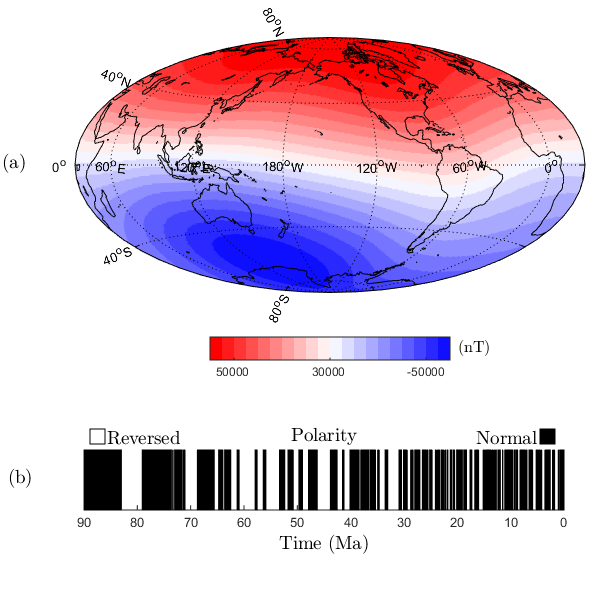
\includegraphics[scale=0.6]{Earth_Field.png}
\caption{(a) Dipolar magnetic field of the Earth in its normal orientation. (b) Polarity of the field inferred from the geological record over the past 90 Ma \cite[]{Cande1995}.}
\label{fig:Earth_Field}
\end{figure}

Natural Remanent Magnetization $\vec M_{NRM}$ is a permanent magnetization moment preserved in the absence of an inducing field.
The reader is encouraged to refer to \cite{Blakely96} and \cite{Clark99} for a more in-depth explanation of chemical, thermal and biological processes responsible for the remanent component of various rock types.
While the induced component is linearly related to the inducing field, nothing can be assumed about the NRM orientation and it remains challenging to estimate.
If aligned with the inducing field direction, the NRM is indistinguishable from a purely induced response, resulting in an over-estimation of the magnetic susceptibility of rocks.
For large NRM components, perpendicular or anti-parallel to the inducing field, the magnetic response of compact objects may get distorted, potentially resulting in false interpretation about the distribution and geometry of rock units.
Direct geological interpretation of magnetic data that ignores the effect of remanence has long been recognized as problem in mineral exploration.
This brings up an important question:
How can we better recover the location and geometry of magnetized objects without knowledge of the total magnetization direction $\vec M$?

From Gauss's law, the relation between the observed magnetic field and rock magnetization is expressed as:
\begin{equation} \label{b_integral}
	\vec b(r) = \frac{\mu_0}{4\pi} \int_{V} \nabla \nabla \frac{1}{ r} \cdot \vec M \; dV\;,
\end{equation}
where $\vec b$ is the magnetic field (T) as measured at some distance $ r$ from a magnetic anomaly with magnetization per unit volume $\vec M$ (A/m).
Since $\vec b$ is usually small, it is commonly measured in units of nano-Tesla (nT).
The majority of magnetic data consist of Total Magnetic Intensity (TMI) measurements which can be written as:
\begin{equation}
	b^{TMI} = |\vec B_0 + \vec B_A| \;,
\end{equation}
where we measure the magnitude of the field rather than the individual components.
In most cases we are only interested in the anomalous local fields.
Under the assumption that $|\vec B_A| \ll |\vec B_0|$, the anomalous field is approximated to be parallel with the direction of the inducing field $\hat B_0$.
The Total Magnetic field Anomaly (TMA) is given by:
\begin{equation}
\begin{split}
	b^{TMA} &= |\vec B_0 + \vec B_A| - |\vec B_0| \\
	&\simeq  \vec B_A \cdot \hat B_0 \;.
\end{split}
\end{equation}
Figure~\ref{fig:Magnetization} gives an example of TMA data measured on a plane above a magnetized sphere.
The main challenge in interpreting magnetic data is to characterize the magnetic sources when nothing is known about the location and magnetic properties ($\kappa,\;\vec M$) of buried objects.
Accurately imaging the location and geometry of magnetic objects is a core problem in exploration geophysics.


\begin{figure}[h!]
\centering
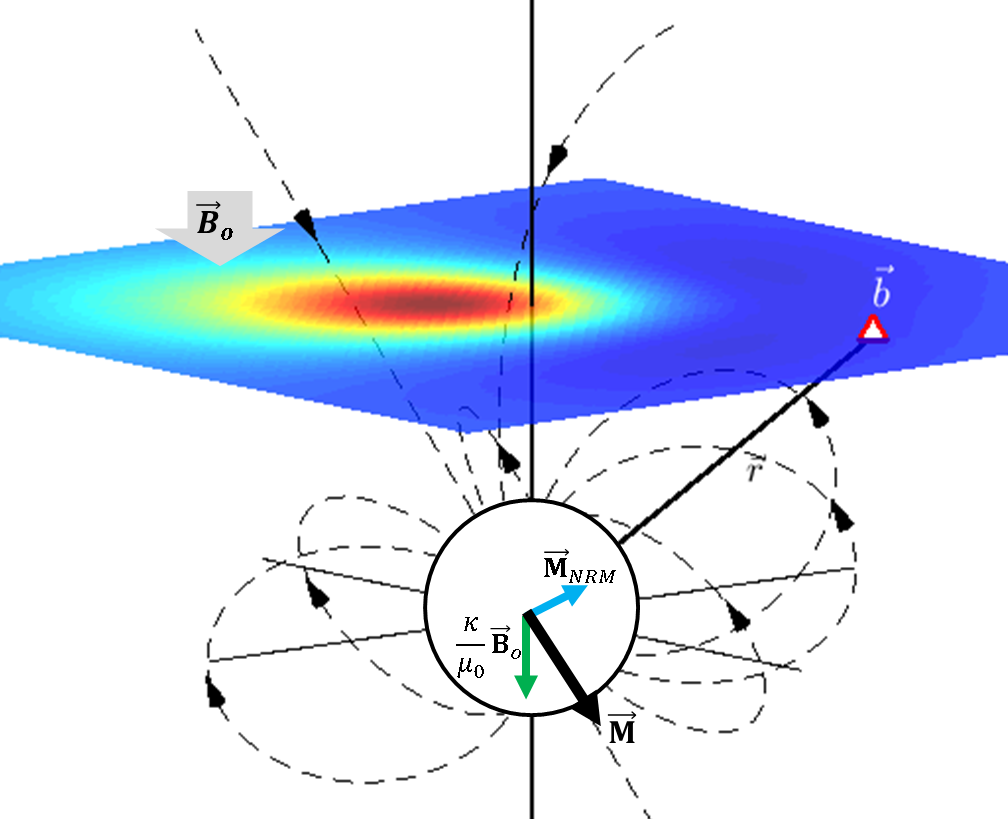
\includegraphics[scale=0.55]{Magnetization_EDT.png}
\caption{Magnetic field data $\vec b$ observed on a plane over a magnetized sphere located at the origin. The orientation and magnitude of magnetization of the sphere is function of the magnetic susceptibility $\kappa$, the inducing field $\vec B_0$ and remanent components $\vec M_{NRM}$, neglecting self-demagnetization effects. }
\label{fig:Magnetization}
\end{figure}

Early geophysical studies relied primarily on filtering techniques to infer geological structures and identify potential targets \cite[]{Cowan2000}.
In order to reduce the complexity of the problem, the magnetization direction is in most cases assumed to be purely induced along $\vec B_0$, neglecting self-demagnetization and remanence effects.
Inversion codes, such as the UBC-MAG3D from \cite{LiOldenburg1996}, also rely on this assumption.
While the induced component may dominate in most cases, recent petrophysical studies seem to indicate that the effect of remanent magnetization may be more important than previously thought \cite[]{Enkin2014}.
This is especially true for specific types of mineral deposits such as Banded Iron-Formations (BIF) and diamondiferous kimberlite \cite[]{Dransfield2003, LiShearer10}
Strong remanent magnetic components can hinder the interpretation of magnetic data thus leading to false drilling targets.

\section{Magnetic methods}
Several studies have been dedicated to the inversion of magnetic data in the presence of remanence.
As summarized by \cite{Li2012}, the proposed inverse methods can be divided into three categories.
The first category estimates the magnetization direction from the data in a pre-processing step.
Strategies such as the Helbig's method \cite[]{Phillips03} and the cross-correlation \cite[]{DannemillerLi06} are used upstream of standard inversion codes.
Adapted from the 2-D analytical signal of \cite{Nabighian72}, \cite{Roest92} estimate the orientation of remanence in 3-D.
In most cases, data are transformed to the wavenumber domain in order to extract magnetic field components.
These methods are simple and robust for simple and isolated anomalies, but become impractical when the data are acquired over rough terrain or complicated geology.

The second category deals with magnetic data that are weakly dependent on the orientation of magnetization.
It has been shown that magnetic amplitude data are weakly dependent on the magnetization direction in 3-D \cite[]{Nabighian72}.
Magnetic amplitude data are simply calculated as:
\begin{equation}
|\vec b| = {( b_x^2 + b_x^2 + b_x^2 )}^{1/2}\;,
\end{equation}
where $b_x$, $b_y$ and $b_z$ are the three components of the anomalous magnetic field.
Inverting magnetic amplitude data can provide a robust estimate for the location of magnetized bodies
as shown by \cite{Shearer05}. Magnetic amplitude data are successfully inverted over a kimberlite deposit, recovering the true location of kimberlite pipes and associated magnetic dykes.
Because most magnetic surveys only record TMI data, the three components of the field must be derived in post-processing.
Two strategies have been proposed in the literature to extract magnetic field components.
The first relies on the fact that magnetic data are potential field data, hence knowledge of any component of the field on an infinite plane above the source is sufficient to calculate the remaining components. 
Data are interpolated onto a uniform grid, which is then used to calculate the components of the field using Fourier transform techniques.
This may be a problem however for airborne surveys over steep topography or acquired at low latitude.
Alternatively, the equivalent-source method has been proposed by \cite{Li2010} to alleviate those constraints.
Taking advantage of the non-uniqueness of potential field data, TMA data are inverted for a layer of magnetic sources then used to forward model three-component magnetic data.


The third method directly solves for the orientation of magnetization without making any assumptions about the location or geometry of causative bodies.
In the Magnetic Vector Inversion (MVI) proposed by \cite{Lelievre2009}, the magnetization vector is decomposed in its induced and orthogonal components.
The MVI is closely related to the method proposed by \cite{Kubota2005}, and later borrowed by \cite{Ellis2012}.
This method results in a large under-determined inverse problem, with roughly three times the number of free-variables over conventional susceptibility inversion codes.
Recovered magnetization models are generally smooth and become overly complicated for direct geological interpretation.
As pointed out by \cite{PhDLelievre09}, any \emph{a priori} information from surface or borehole measurements may greatly reduce the non-uniqueness of the problem.
Unfortunately this kind of information is rarely available in greenfield settings or is only available in sparse samples.

Building upon the work of \cite{Shearer05}, \cite{Liu2015} propose a hybrid three-step process to invert for the location, orientation and magnetic susceptibility distribution in 2-D.
In the first step, the location of magnetic material is inverted from amplitude data.
Next, the orientation of magnetization is found via a correlation method.
The orientation of magnetization is then used in a standard inversion code to recover a susceptibility model.
The combined method greatly reduces ambiguity about the location and orientation of isolated targets, but becomes challenging over multiple anomalies with variable magnetization directions.
The same synthetic model was applied to the MVI method, resulting in a poor recovery for the location and intensity of magnetization.
This result is surprising considering the satisfactory solution obtained in previous studies \cite[]{Ellis2012, Lelievre2009}.
The combined approach of \cite{Liu2015} is interesting however, as it links together complementary algorithms.

\section{Thesis outline}
Following the same line of thought as \cite{Liu2015}, I propose a Cooperative Magnetic Inversion (CMI) algorithm that directly incorporates the amplitude inversion of \cite{Shearer05} into the MVI algorithm of \cite{Lelievre2009}.
Magnetic field amplitude data are computed from the Equivalent Source technique proposed by \cite{Li2010}, removing the need to grid the data.
Moreover, I introduce a Scaled Iterative Re-weighted Least Squares (S-IRLS) regularization method to recover blocky and sparse solutions.
My thesis is divided into the following chapters:

In Chapter~\ref{ch:Chap2_Forward} and \ref{ch:Chap3_Inverse}, I provide further details about rock magnetism and review the theory related to inverse problems in the context of exploration geophysics. I revisit three inversion codes from the literature: the magnetic susceptibility inversion from \cite[]{LiOldenburg1996}, the magnetic amplitude inversion from \cite{Shearer05}, and the Magnetic Vector Inversion (MVI) from \cite[]{PhDLelievre09}.
Each of these codes are tested on a synthetic example with complicated magnetization distribution.
I also review the equivalent-source method from \cite{Li2010}.

In Chapter~\ref{ch:Chap4_Mixed_Lpnorm_Regularization}, I introduce a mixed $l_p$-norm regularization function for the recovery of compact and sparse solutions, increasing the flexibility of current inversion codes.
The method uses a Scaled Iterative Re-weighted Least Squares (S-IRLS) formulation to approximate any $l_p$-norm penalties on the interval $0 \le p \le 2$.
Sparse constraints are applied on both the model and model gradients independently.
The mixed-norm regularization is implemented on the magnetic problem, and tested on an airborne magnetic dataset from the Tli Kwi Cho kimberlite complex, Northwest Territories.

In Chapter~\ref{ch:Chap5_Cooperative_Mag_Inversion_CMI}, I formulate a Cooperative Magnetic Inversion (CMI) method, combining the inversion codes presented in Chapter~\ref{ch:Chap3_Inverse} and \ref{ch:Chap4_Mixed_Lpnorm_Regularization}.
The algorithm is tested on the same synthetic example for comparison.

Finally in Chapter~\ref{ch:Chap6_Case_Study}, I apply the CMI algorithm to a large aeromagnetic data set over the Ekati Property, Northwest Territories.
I design a tiled inversion scheme to automate the inversion process and to reduce the computational cost.
Individual models are then merged back onto a global mesh for analysis.
A bulk estimate of magnetization direction is compared to values published in the literature.
The polarities of magnetization over 11 pipes are compared to the estimated age of emplacement.
The analysis is extended to various dyke swarms, providing regional geologic information.

The work presented in this thesis is significant for two reasons.
First, the mixed-norm regularization function introduced in Chapter~\ref{ch:Chap4_Mixed_Lpnorm_Regularization} can considerably improve the flexibility of inversion algorithms, not limited to potential field problems.
The S-IRLS method allows for a combination of sparse norms on the model and model gradients independently, granting access to a wider range of solutions than previously offered by globally convex functions.
%Future research will focus on the implementation of the S-IRLS on other geophysical inverse problems such as for gravity and electromagnetic data.

Secondly, it is the first time that both the amplitude inversion and MVI algorithms are combined in a cooperative inversion method in 3-D.
Structural information gained by the amplitude inversion is used directly to constrain the MVI algorithm, reducing the non-uniqueness of the solution.
From a practical standpoint, it is an automated process that streamlines the inversion workflow.
This, in turn, can reduce the overall time required to process magnetic data and promote the expansion of inversion methods in mineral exploration.
%Future research will focus on the implementation of a non-linear spherical formulation for the MVI, improving the flexibility of the algorithm.

\endinput

